\documentclass[10pt]{beamer}

\usetheme{metropolis}
\usepackage{appendixnumberbeamer}

\usepackage{booktabs}
\usepackage[scale=2]{ccicons}

\usepackage{pgfplots}
\usepgfplotslibrary{dateplot}

\usepackage{caption}
\captionsetup[figure]{font=scriptsize,labelfont=scriptsize}

\usepackage{xspace}
\newcommand{\themename}{\textbf{\textsc{metropolis}}\xspace}

% Bibliography font size
\setbeamerfont{bibliography item}{size=\footnotesize}
\setbeamerfont{bibliography entry author}{size=\footnotesize}
\setbeamerfont{bibliography entry title}{size=\footnotesize}
\setbeamerfont{bibliography entry location}{size=\footnotesize}
\setbeamerfont{bibliography entry note}{size=\footnotesize}


% No "Figure x:" caption
\usepackage{caption}
\captionsetup[figure]{labelformat=empty}

\title{A Big Data Analytics Framework for Evaluating Automated Elastic Scalability of the SMACK-Stack}
\subtitle{Diploma Examination}
\date{October 25, 2018}
\author{Benedikt Wedenik}
\titlegraphic{%
    \parbox[c]{3cm}{
\includegraphics[width=1.7cm]{img/logo_institut}}
    \hspace*{4.5cm}
    \parbox[c]{3cm}{
\includegraphics[width=2.5cm]{img/logo}}
}



%\setbeamertemplate{frame footer}{Benedikt Wedenik - 1227151}

\begin{document}

\maketitle

\begin{frame}{Table of contents}
  \setbeamertemplate{section in toc}[sections numbered]
  \tableofcontents[hideallsubsections]
\end{frame}

%%%%%%%%%%%%%%%%%%%%%
\section{Motivation \& Research Challenges}
%%%%%%%%%%%%%%%%%%%%%

\begin{frame}{Motivation}
	In the last years the demand for information availability and shorter response times has been increasing.
	Today's business requirements are changing: Waiting hours or even days for the result of a query is not acceptable anymore in many sectors.\\

	The response needs to be immediate, or the query is discarded \cite{estrada2016big}.
	This is why "Fast Data", as an approach to solve those problems, increases its popularity, as being "big data, but fast" \cite{mishne2013fast}.\\
\end{frame}

\begin{frame}{Research Challenges}
	\begin{itemize}
	\item \textbf{Deploying large scale applications} \\
		Requires multiple instances of different technologies to be deployed in a defined sequence to fulfill subsequent dependencies, often including manual steps.
	\item \textbf{Initial setup} \\
		The decision of how to configure the instances of an application is a non-trivial task, as there are almost infinite combination possibilities and the impact can be drastic.
	\end{itemize}
\end{frame}

\begin{frame}{Research Challenges}
	\begin{itemize}
	\item \textbf{Monitoring} \\
		Considering just RAM, CPU and disk usage is in most cases insufficient, as a deeper understanding of the used frameworks is required, which introduces a new layer of complexity.
	\item \textbf{Scaling when needed} \\
		Understanding what’s going on in a cluster and reacting accordingly is crucial for the success of any large scale application.
	\end{itemize}
\end{frame}

%%%%%%%%%%%%%%%%%%%%%%%
\section{Background}
%%%%%%%%%%%%%%%%%%%%%%%

\begin{frame}{Background}
		The SMACK-Stack consists of five technologies combined to a lightning fast data pipeline for today's needs of big data applications, as shown below.\\
        \hfill
		\begin{figure}[!htbp]
  			\centering
  			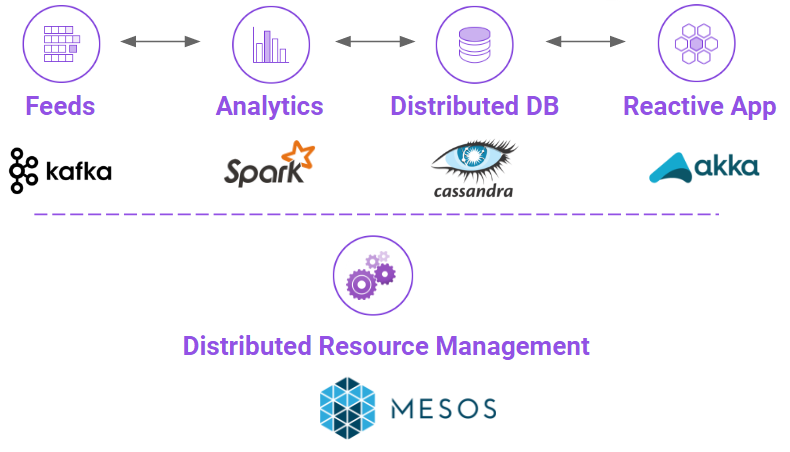
\includegraphics[keepaspectratio=true,width=9cm]{img/smack_stack}
                \caption{mesosphere.com \cite{mesosphere}}
  			\label{fig:smack_stack}
		\end{figure}
\end{frame}

\begin{frame}{Background}
		\begin{itemize}
 		 \item Apache \textbf{S}park is the engine of the pipeline, providing batch-, as well as stream-processing power for large-scale data processing.
   		 \item \textbf{M}esos is a datacenter operating system with the aim to reduce complexity and ease the deployment and maintenance of large-scale distributed applications.
   		 \item Apache \textbf{A}kka can be seen as the model, providing the possibility to build powerful reactive distributed message-driven applications.
		\end{itemize}
\end{frame}

\begin{frame}{Background}
		\begin{itemize}
   		 \item Apache \textbf{C}assandra is a highly distributed database which is a hybrid between a column-oriented and a key-value DBMS, which is implemented avoiding a single point of failure.
   		 \item Apache \textbf{K}afka serves as publish-subscribe message broker, which is usually the ingestion point of the pipeline.
		\end{itemize}
\end{frame}

%%%%%%%%%%%%%%%%%%%%%
\section{Contribution}
%%%%%%%%%%%%%%%%%%%%%

\begin{frame}{Contribution}
	To solve the mentioned problems, a framework has been developed, whereas the single components can be described as follows:\\
	\hfill \\

	\begin{itemize}
   	 \item \textbf{Framework to Easily Launch SMACK in AWS}\\
          With the help of this framework it takes just a few command line calls to launch and deploy the whole SMACK stack in the cloud.
  	  \item \textbf{JMX Extraction Tool}\\
          This tool is designed to automatically extract interesting metrics from SMACK components via JMX and sending them to a central service, in this case the REST monitoring service.
	\end{itemize}
\end{frame}

\begin{frame}{Contribution}
	\begin{itemize}
   	 \item \textbf{REST Service Collecting Monitoring Information}\\
          This is the service which collects all the extracted metrics and compiles them into a useful format.
          In addition, there is the possibility to generate plots at runtime.
  	  \item \textbf{Automated Scaling Tool for SMACK}\\
          The scaling tool evaluates the collected metrics from the REST service and scales the individual parts of the SMACK stack up or down.
   	 \item \textbf{Deployment Blueprints}\\
          Those reference architecture and configuration recommendations help to launch the SMACK stack and getting most out of the available resource.
	\end{itemize}
\end{frame}

{ % all template changes are local to this group.
    \setbeamertemplate{navigation symbols}{}
    \begin{frame}[plain]
        \begin{tikzpicture}[remember picture,overlay]
            \node[at=(current page.center)] {
                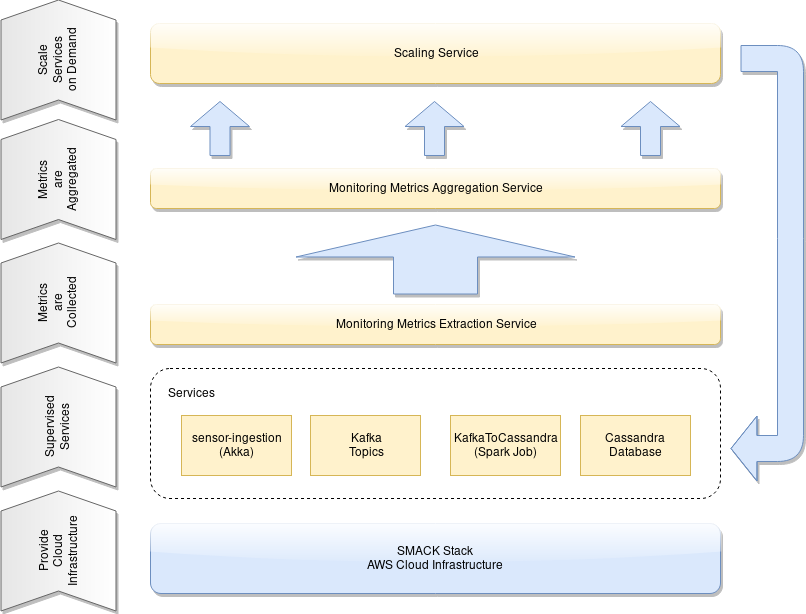
\includegraphics[width=12cm]{img/architecture}
            };
        \end{tikzpicture}
     \end{frame}
}

%%%%%%%%%%%%%%%%%%%%%%%
\section{Evaluation}
%%%%%%%%%%%%%%%%%%%%%%%
\begin{frame}{Evaluation}
In order to evaluate the framework's performance, a use-case based approach with two real-world applications is chosen.\\
As part of the contribution, two real world applications have been developed in order to provide a valid base for the evaluation of the framework.
\hfill

    \begin{itemize}
        \item The \textit{IoT Data Storage Application} is mainly I/O bound and represents applications which require high throughput.
        \item In case of the \textit{Acceleration Prediction Application}, a prediction based on IoT data is performed, which is heavily computational intense.\\
    \end{itemize}
\end{frame}

{ % all template changes are local to this group.
    \setbeamertemplate{navigation symbols}{}
    \begin{frame}[plain]
        \begin{tikzpicture}[remember picture,overlay]
            \node[at=(current page.center)] {
                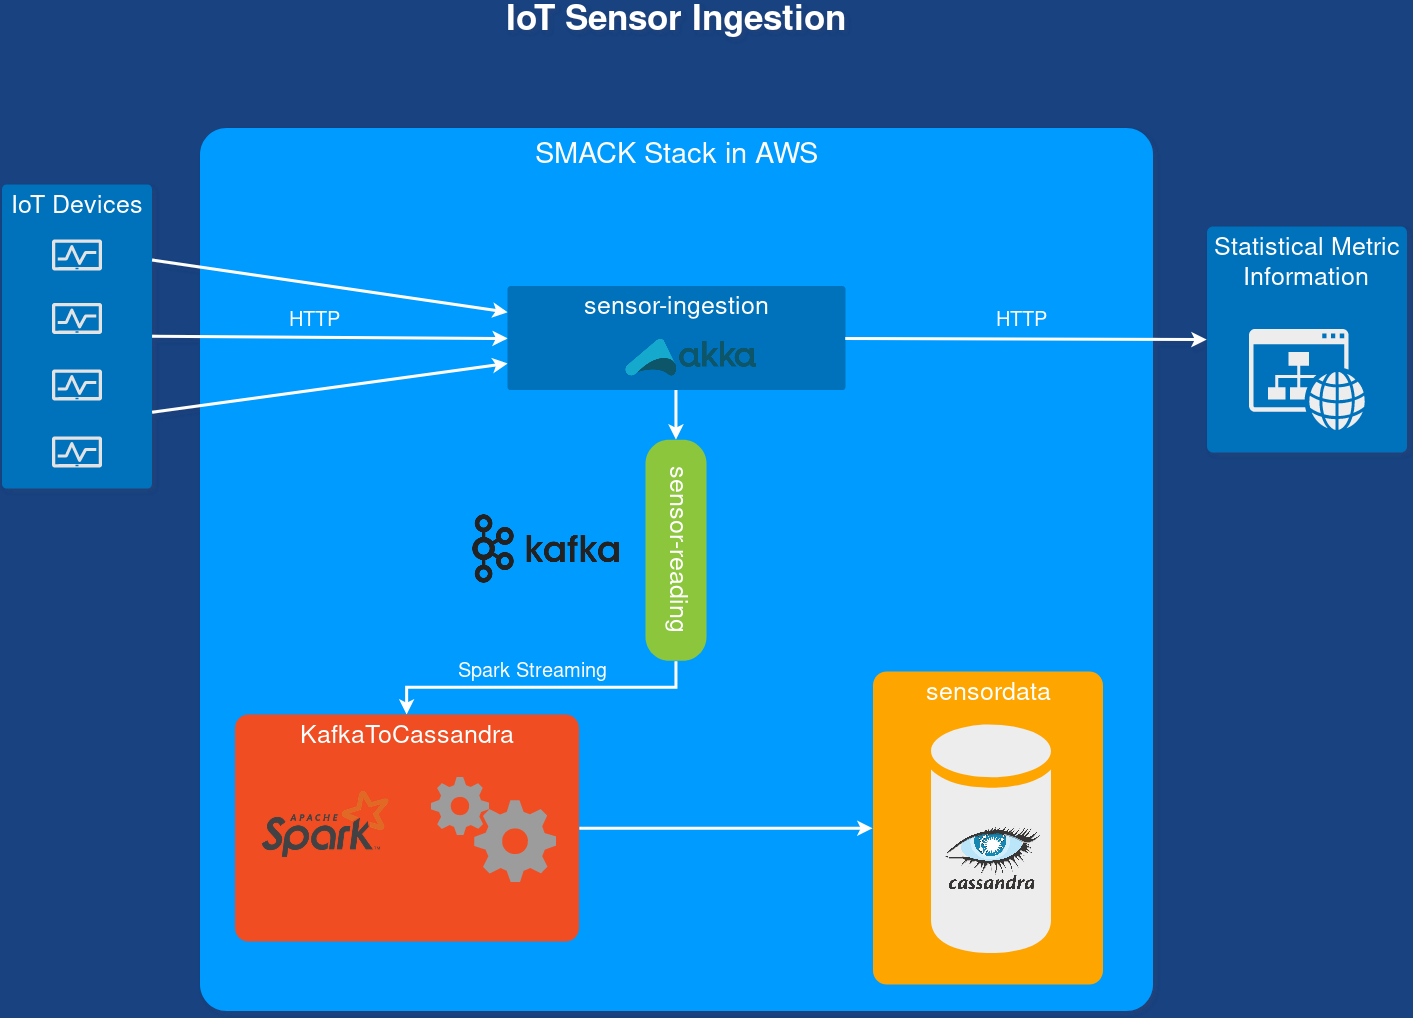
\includegraphics[width=11cm]{img/IoT}
            };
        \end{tikzpicture}
     \end{frame}
}

{ % all template changes are local to this group.
    \setbeamertemplate{navigation symbols}{}
    \begin{frame}[plain]
        \begin{tikzpicture}[remember picture,overlay]
            \node[at=(current page.center)] {
                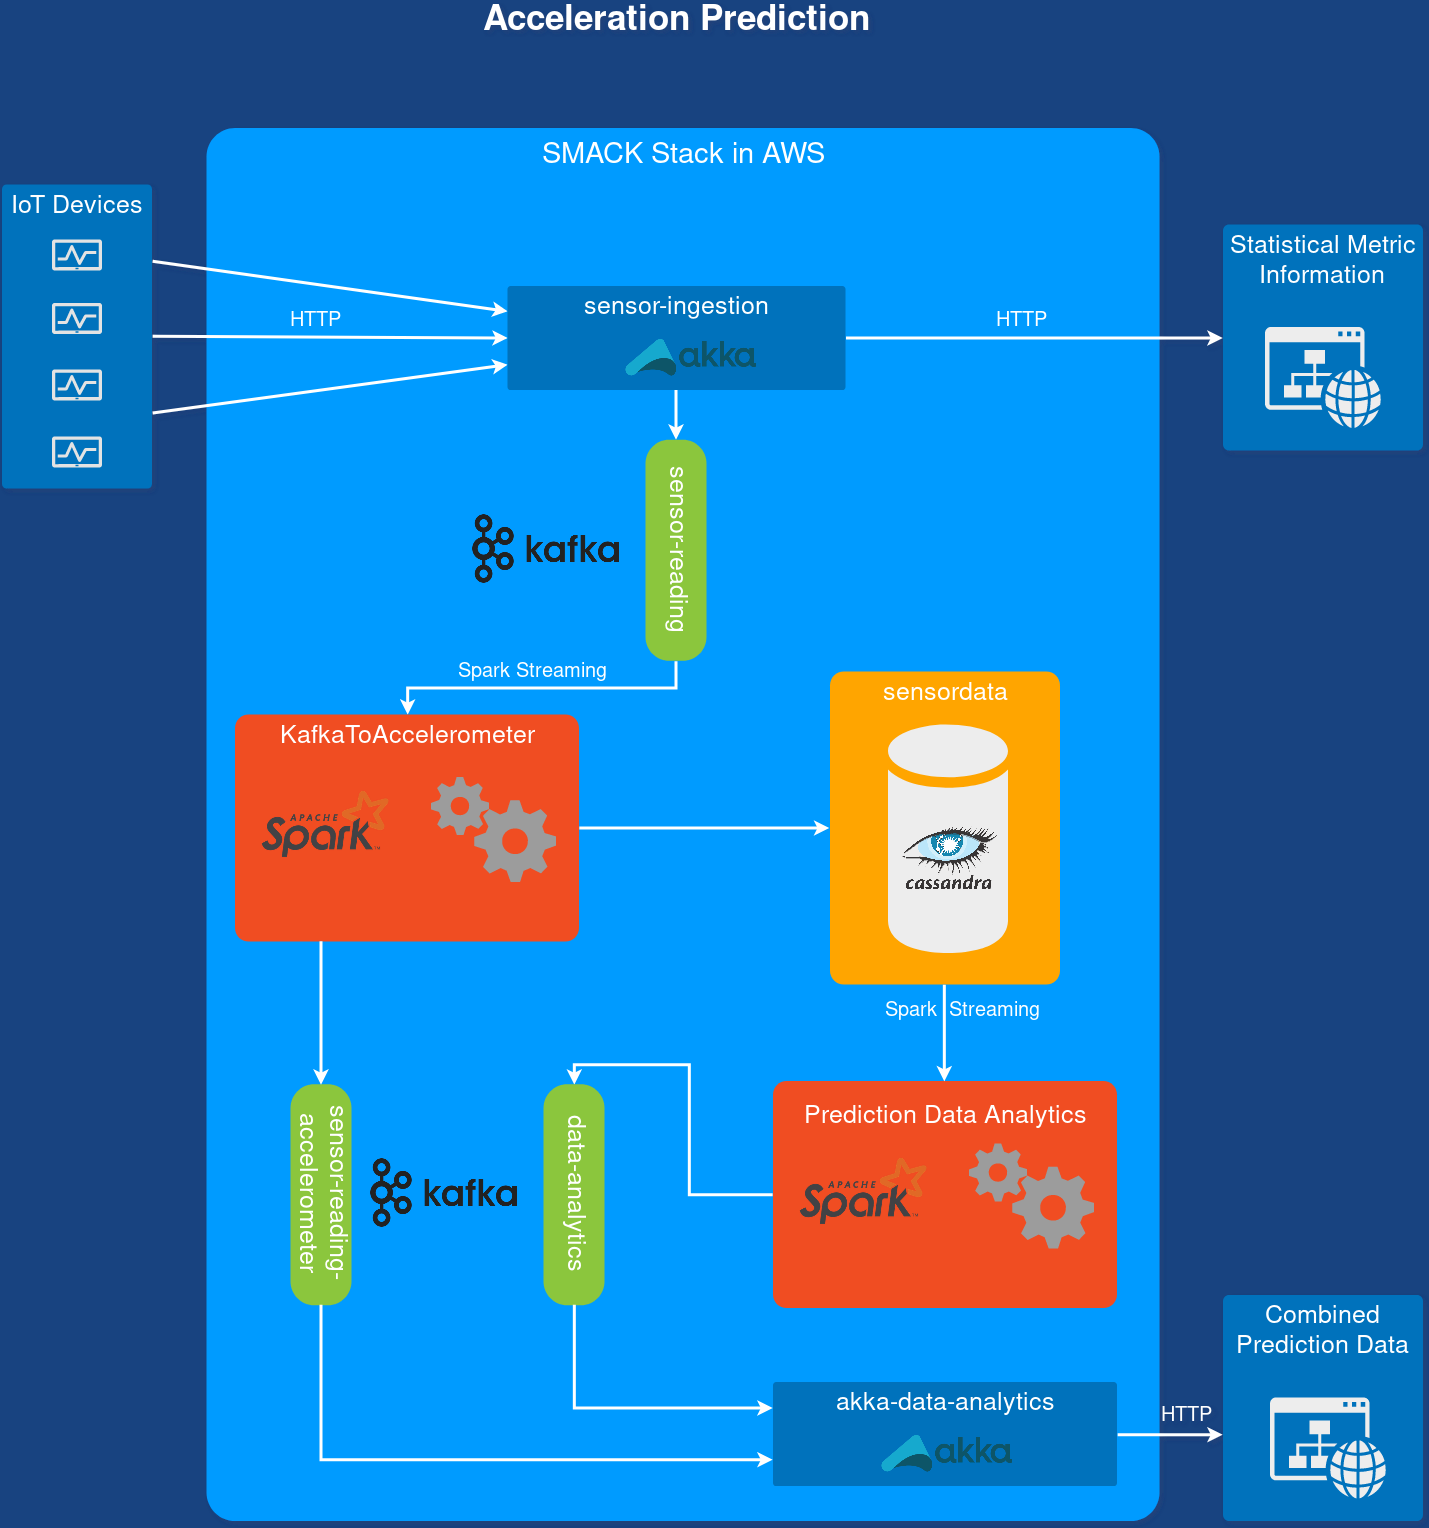
\includegraphics[width=8.5cm]{img/prediction}
            };
        \end{tikzpicture}
     \end{frame}
}

{ % all template changes are local to this group.
    \setbeamertemplate{navigation symbols}{}
    \begin{frame}[plain]
        \begin{tikzpicture}[remember picture,overlay]
            \node[at=(current page.center)] {
                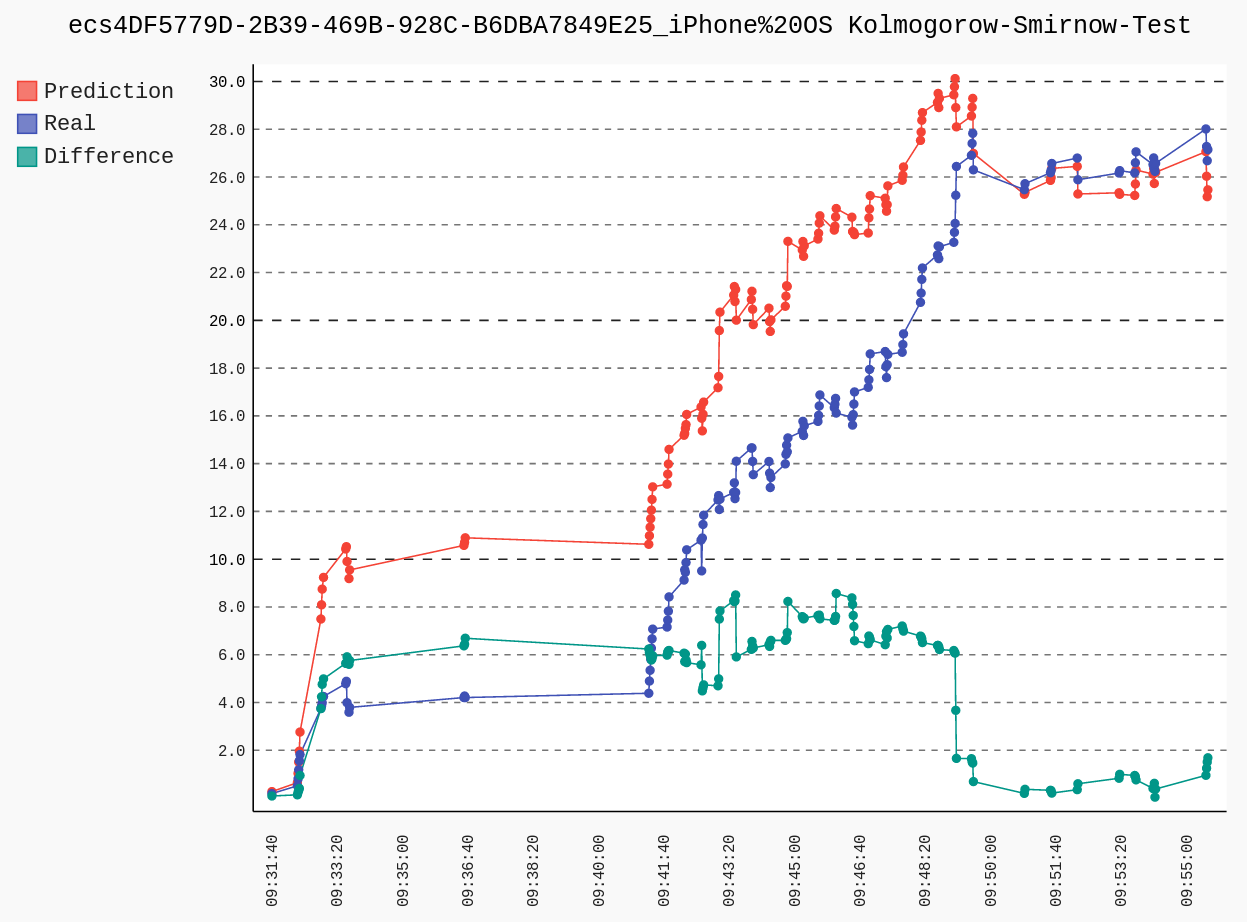
\includegraphics[width=10cm]{img/prediction_vs_real}
            };
        \end{tikzpicture}
     \end{frame}
}

{ % all template changes are local to this group.
    \setbeamertemplate{navigation symbols}{}
    \begin{frame}[plain]
        \begin{tikzpicture}[remember picture,overlay]
            \node[at=(current page.center)] {
                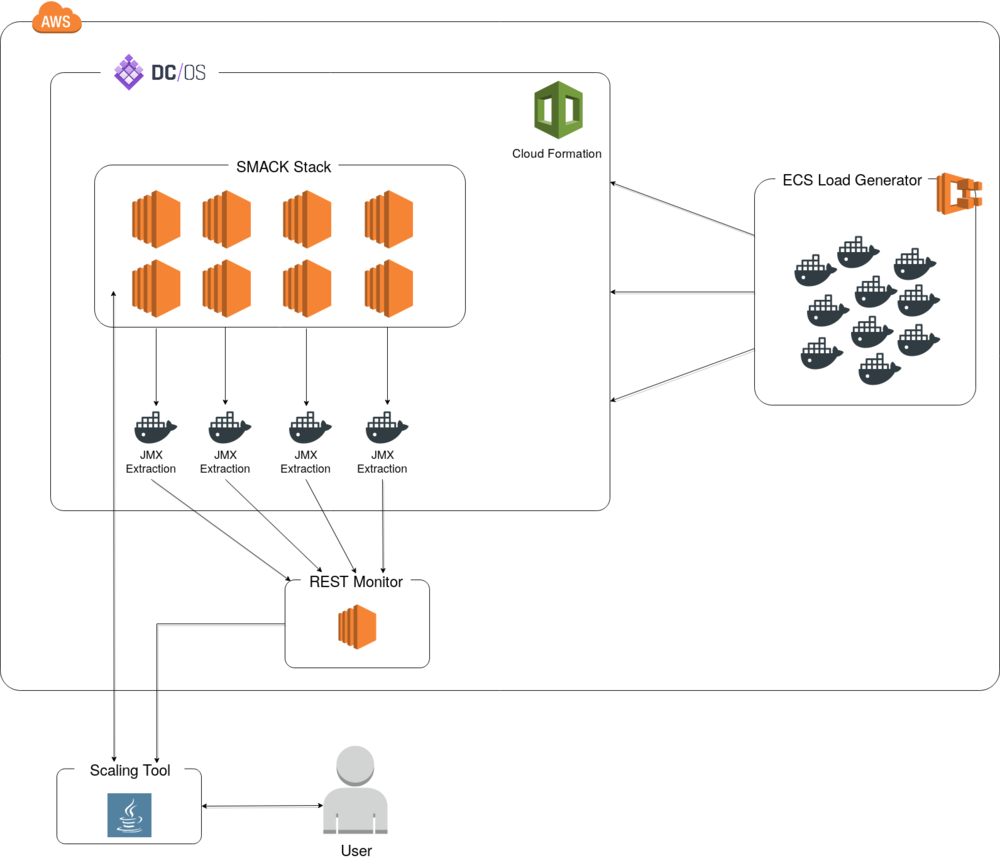
\includegraphics[width=10cm]{img/overall_view}
            };
        \end{tikzpicture}
     \end{frame}
}

%%%%%%%%%%%%%%%%%%%%%%%
\section{Results \& Conclusion}
%%%%%%%%%%%%%%%%%%%%%%%
\begin{frame}{Results}
	Empirical experiments have been conducted for evaluation.\\
    The setup comprises two runs: \textbf{unsupervised}, which serves as a baseline,\\
    and \textbf{supervised}, in which the framework automatically scales the respective services.\\
	Both applications benefit from the scaling service, where the following improvements can be highlighted:\\
    \hfill

	\begin{itemize}
		\item An \textbf{increase from 272 to 472 MBit/s} was measured when running the \textit{IoT Data Storage Application}, as well as other \textbf{metrics like the time-in-mailbox of a message were improved}.
		\item The \textit{Acceleration Prediction Application} benefited in form of \textbf{shorter message processing times} and an overall \textbf{faster task completion}.
              Based on the calculated average of the task completion, the run with the enabled Scaling Tool was about 169\% faster.
	\end{itemize}
\end{frame}

{ % all template changes are local to this group.
    \setbeamertemplate{navigation symbols}{}
    \begin{frame}[plain]
        \begin{tikzpicture}[remember picture,overlay]
            \node[at=(current page.center)] {
                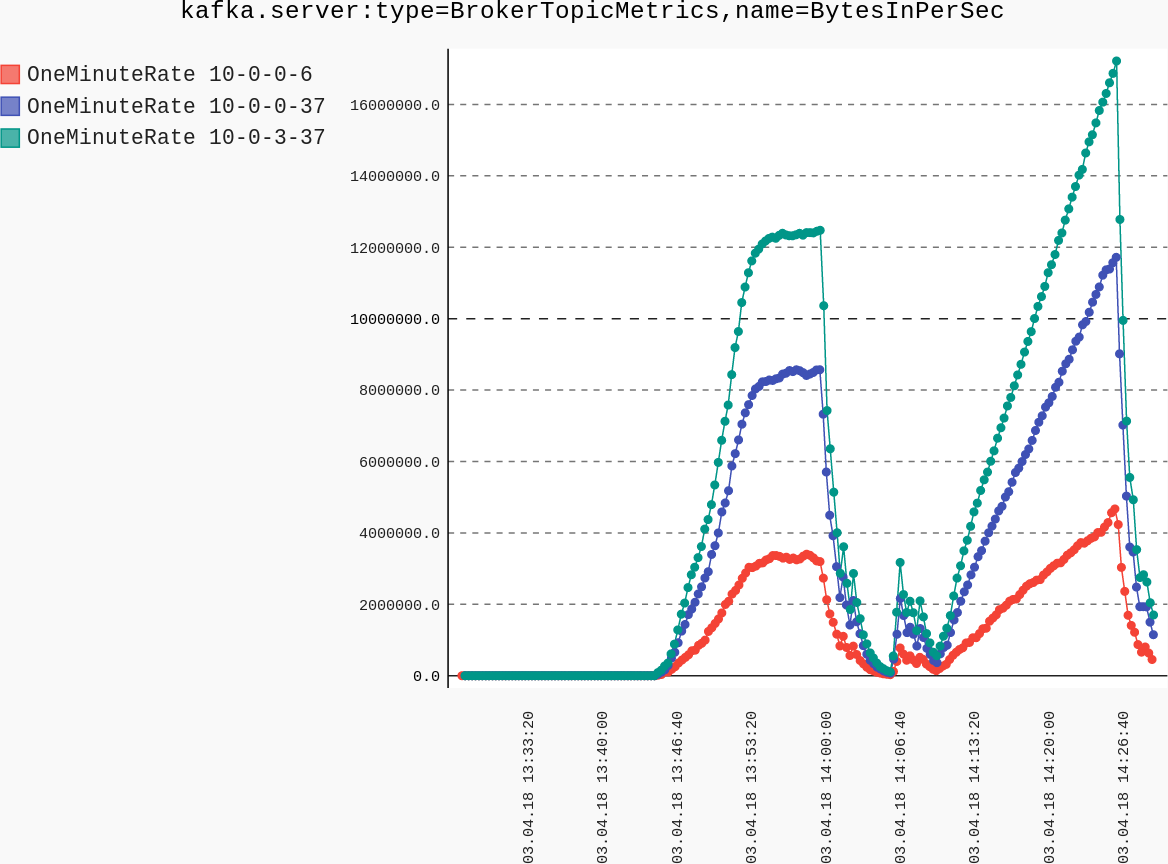
\includegraphics[width=12cm]{img/before_kafka_bytes_in_separate}
            };
        \end{tikzpicture}
     \end{frame}
}

{ % all template changes are local to this group.
    \setbeamertemplate{navigation symbols}{}
    \begin{frame}[plain]
        \begin{tikzpicture}[remember picture,overlay]
            \node[at=(current page.center)] {
                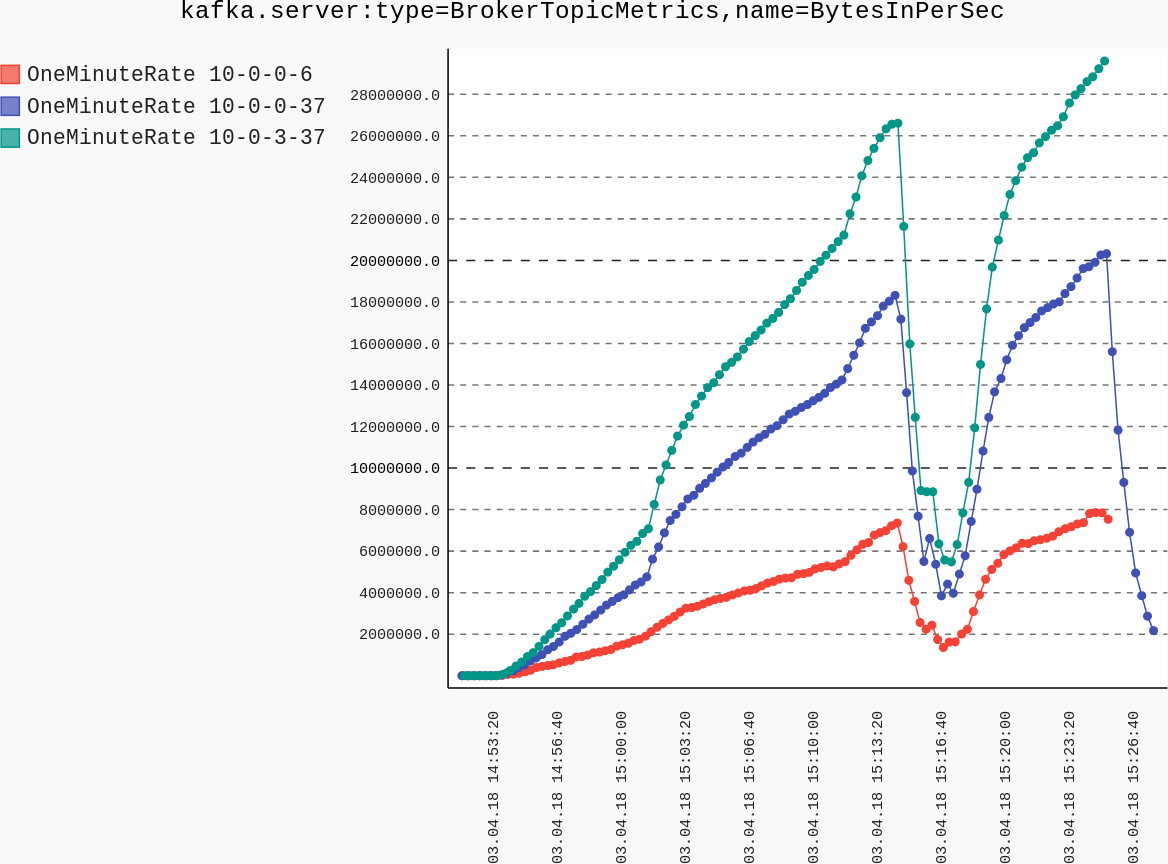
\includegraphics[width=12cm]{img/after_kafka_bytes_in_separate}
            };
        \end{tikzpicture}
     \end{frame}
}

{ % all template changes are local to this group.
    \setbeamertemplate{navigation symbols}{}
    \begin{frame}[plain]
        \begin{tikzpicture}[remember picture,overlay]
            \node[at=(current page.center)] {
                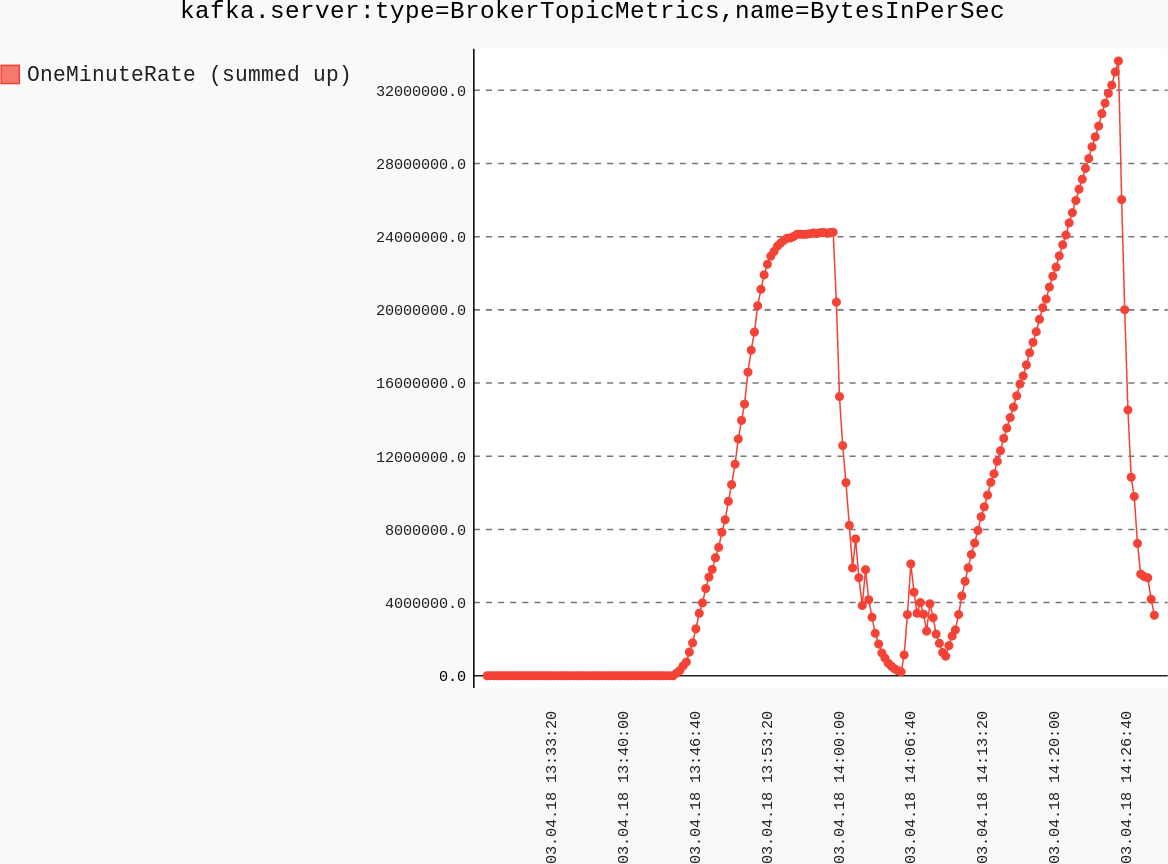
\includegraphics[width=12cm]{img/before_kafka_bytes_in_sum}
            };
        \end{tikzpicture}
     \end{frame}
}

{ % all template changes are local to this group.
    \setbeamertemplate{navigation symbols}{}
    \begin{frame}[plain]
        \begin{tikzpicture}[remember picture,overlay]
            \node[at=(current page.center)] {
                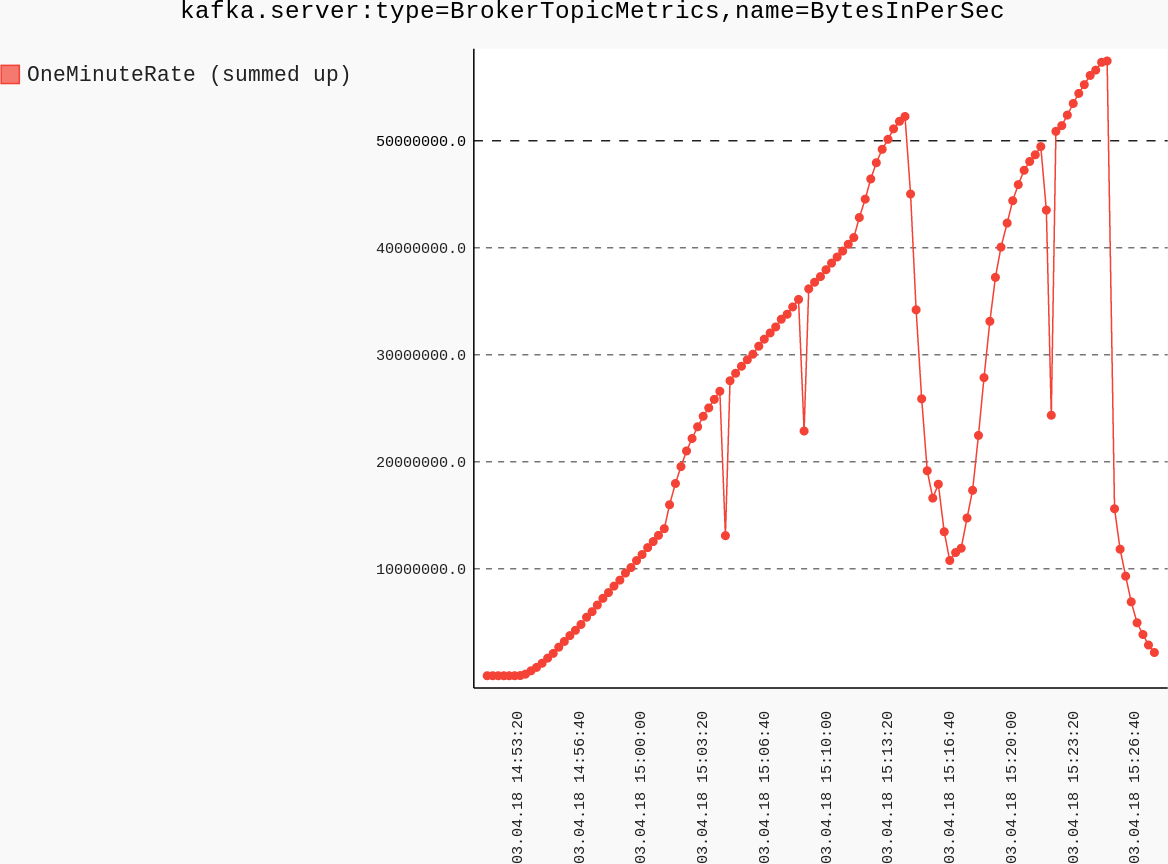
\includegraphics[width=12cm]{img/after_kafka_bytes_in_sum}
            };
        \end{tikzpicture}
     \end{frame}
}

\begin{frame}{Open Issues \& Future Work}
    \begin{itemize}
        \item Kolmogorov Smirnov test shows, that the prediction correlates with the real measured values. Still there is an obvious bias, which could be eliminated or at least decreased.
        \item Extended REST API for Acceleration Prediction Application.
        \item Unfortunately scaling down is not supported for Kafka and Cassandra, due to the restrictions of DC/OS \cite{mesosphere}, \cite{cassandra_limitations}.
        \item The selection of what to extract could be refined further to reduce overhead and only focus on what is important.
        \item Currently the threshold management in the Scaling Tool is hard-coded and static, which is an obvious place for further improvements.
    \end{itemize}
\end{frame}

%%%%%%%%%%%%%%%%%%%%%%%
\section{Questions}
%%%%%%%%%%%%%%%%%%%%%%%


\begin{frame}[standout]
  I'm happy to answer your questions!
\end{frame}

\begin{frame}
      \begin{block}{References}
		\begin{footnotesize}
			\bibliographystyle{abbrv}
            \bibliography{cites}
		\end{footnotesize}
      \end{block}
\end{frame}


\end{document}

